% CS 217A/B, Winter/Spring 2017
% Professor Lixia Zhang
% Project Final Report

\documentclass{sig-alternate}

% General packages and setup
\PassOptionsToPackage{hyphens}{url}\usepackage{hyperref}  % For embedding clickable links to citations
\paperheight=11in
\renewcommand\_{\textunderscore\allowbreak}  % Allows line breaks on words with underscores

\usepackage{listings}

\begin{document}
	
\title{ndnMouse\\Secure Control Interface for a PC Using a Mobile Device}
%\subtitle{CS 217B Project Final Report, Spring 2017}
\subtitle{Master's Capstone Project Report}
\numberofauthors{1}
\author{
	Wesley Minner\\
	Computer Science M.S. Student\\
	wesleyminner@gmail.com
}

\date{18 May 2017}
\maketitle

% ==============================================================================
\begin{abstract}
This report outlines the results of my efforts on ndnMouse, my Master's Capstone project, as well as my class project for CS 217B. It is open-sourced on Github~\cite{ndnMouseGH} under the GNU public license, and available on the Google Play App Store~\cite{ndnMouseGP}. The goal of ndnMouse is to securely and efficiently control one or more personal computers via remote mouse movement and rudimentary keyboard commands from your phone, running the communication protocol over Named Data Networking (NDN)~\cite{ndn}. In order to judge the design and performance benefits of NDN, ndnMouse also supports communication over UDP. Implementation of both protocols resulted in fairly unique server and clients designs. The pros and cons of each will be explored in this report.

Section 1 will review the features and use cases of ndnMouse, with more detail of the command protocol in Section 2. Details on the security features will be given in section 3, with challenges and trade-offs I have overcome listed in section 4. Performance analysis comparing NDN and UDP implementations is in section 5. Section 6 explores extensions and future use cases for ndnMouse, and finally section 7 concludes this report. Additionally screenshots of the application are in section 9, the Appendix.
\end{abstract}


\keywords{NDN, Mouse, Keyboard, Remote Access, Security}

% ==============================================================================
\section{Overview}
NdnMouse provides remote access to the mouse and keyboard of a PC in order to provide a simple and convenient way to wirelessly interface with your computer from across the room. Wireless slideshow/powerpoint control represented the main use case, removing the need for a proprietary piece of hardware (such as a USB/bluetooth clicker device). Anecdotal evidence suggests that users of these devices encounter a variety of issues such as: drained batteries, poor connection, and general hardware failure. Additionally a presenter must also carry around the clicker hardware, which has no other purpose than slideshow control. NdnMouse removes the need for a specialized clicker and adds remote slideshow control to something most people already carry around in their pockets, a smart phone. 

By taking advantage of the local WiFi access point or the phone's WiFi hotspot feature, a user can use their Android smart phone as a virtual touchpad and simple keyboard, providing the functionality needed to step through a powerpoint presentation without any additional hardware. NdnMouse also may be of use during times of hardware failure, providing an emergency backup mouse or keyboard when the user has limited options to interface with their PC.

Both NDN and UDP/IP transport/routing protocols are supported, encrypting packets with AES if a password is provided by the user. Additionally NDN can provide some extra features in the form of interest (query) condensing, allowing the phone server to better scale its performance when multiple PC clients are connected. More on this idea will be described in Section 5. However the protocol choice should ideally be transparent to the user, as all features are supported on both NDN and UDP.

\subsection{Features}
NdnMouse supports full mouse control: relative cursor movement, left click, right click, and a shortcut allowing tap-to-click on the touchpad. Sensitivity and precision settings are also provided, for fine tuning the feel of the movement. Two-finger scrolling works similarly to Apple laptops, with inversion and sensitivity settings as well. Rudimentary keyboard support allows the user to execute common slideshow control commands, such as using the arrow keys or the spacebar to easily change slides. Additionally custom typed messages are supported, allowing the user to type any message using the built-in Android keyboard. Upon sending the message, all receiving client PCs will then virtually the characters out instantly on whatever program window is selected at that time.

The security for ndnMouse was designed to defend against packet snooping, replay attacks, privacy attacks, and brute force attacks. More details will be given in section 3. The user may also choose to not use a password, which sends the communication protocol in cleartext and avoids a minor amount of encryption/decryption overhead. 

\subsection{Supported Platforms}
NdnMouse is composed of two applications: the server/producer Java application (running on the Android phone), and the client/consumer Python application (running on the PC). Any relatively modern Android phone is supported (Android 4.1 and up), and basically any PC that can run NDN's Network Forwarding Daemon (NFD)~\cite{nfd} and Python3~\cite{python3}. Since Python runs on the three major operating systems (Linux, OSX, and Windows), the limiting factor is NFD, which only currently runs on Linux and OSX. However Windows PCs can still use ndnMouse by limiting their protocol choice to UDP only.

Other dependencies include a few Python libraries needed for the PC client, specifically PyAutoGUI~\cite{pyautogui}, PyCrypto~\cite{pycrypto}, and PyNDN~\cite{pyndn}. PyAutoGUI provides mouse and keyboard control, as well as some simple dialog boxes for collecting user input. PyCrypto handles all the cryptography operations, and PyNDN provides the API for using NDN and for interfacing with NFD. The Android application uses jNDN~\cite{jndn} to access the NDN API, but this library comes compiled into ndnMouse's APK and requires no outside installation by the user. Both the PC and Android phone must have NFD installed and running to communicate over NDN.

\section{Protocol}
NdnMouse can run its communication protocol four different ways, depending on the transport protocol used (UDP or NDN) and if a password is provided by the user (security on or off).

\subsection{UDP}
Without a password (all security off), packets are transmitted in cleartext and are at most 16 bytes. UDP uses connection-oriented communication by having the client send an \texttt{OPEN} message to the server, similar to a TCP \texttt{SYN} packet. This asks the server to establish a \textit{session} between the client and itself. An \texttt{OPEN-ACK} reply message is used to respond to the \texttt{OPEN} message and completes the connection setup.

Once a session is established, the server will send unsolicited mouse commands\footnote{I will refer to all commands ndnMouse can send as mouse commands, though this includes supported keyboard commands as well.} to its clients. The data format is not strict across all possible mouse commands, but generally takes the form of one character dictating the type of command, followed by any additional information for that command. For example, a mouse movement command is of the form \texttt{M<x-4B><y-4B>}. I denote the \textit{x} and \textit{y} coordinates each have a fixed length of 4 bytes by appending "\texttt{4B}." See \hyperlink{tab:msgFormat}{Table 1} for the supported, non-secure message formats.

\begin{table}
	\hypertarget{tab:msgFormat}{}
	\begin{center}
		\begin{tabular}{| l | l |}
			\hline
			Message Type & Message Format\\ \hline\hline
			Movement & \texttt{M<x-4B><y-4B>}\\ \hline
			Click & \texttt{C<click\_message>}\\ \hline
			Scroll & \texttt{S<x-4B><y-4B>}\\ \hline
			Keyboard & \texttt{K<keyboard\_message>}\\ \hline
			Typestring & \texttt{T<type\_string-10B-max>}\\ \hline
		\end{tabular}
		\caption{Non-secure message formats}
	\end{center}
\end{table}

Heartbeat messages are sent once every one second to keep the connection alive when no other mouse command packets are being sent. The client query packet contains the message \texttt{HEART}, and the server reply contains the message \texttt{BEAT}. The main goal of heartbeats was to detect when the server had lost its session with the client, such as during a server reset or crash. In these cases, the client would miss a certain number of heartbeat replies from the server, triggering a session restart on the client side. The client would then try to open a new session using \texttt{OPEN} messages. After receiving a \texttt{OPEN-ACK}, the session would resume normal activity.

Lastly a \texttt{CLOSE} message is sent by the client upon exiting the application. This lets the server know that it can stop sending unsolicited mouse command messages. Note that reliable delivery and in-order processing of packets is not needed for ndnMouse, letting the application take advantage of the simplicity and performance of UDP. The simple, connection-oriented communication I implemented on top of UDP allows ndnMouse to gracefully recover from server/client connection problems.

When security features are turned on, the UDP communication protocol becomes slightly more complex to prevent specific types of malicious attacks. Both the packet format and the payload message require changes. In \hyperlink{tab:secureMsgFormat}{Table 2}, the secure message formats are listed. A four byte sequence number is added to the front of each message, and then the entire message will then be encrypted, as described in the section 2.3 on Mouse Packets. The message length is also fixed to 16 bytes, using PKCS5 padding~\cite{rfc8018}.

\begin{table}
	\hypertarget{tab:secureMsgFormat}{}
	\begin{center}
		\begin{tabular}{| l | l |}
			\hline
			Message Type & Secure Message Format\\ \hline\hline
			Movement & \texttt{<seq-4B>M<x-4B><y-4B>}\\ \hline
			Click & \texttt{<seq-4B>C<click\_message>}\\ \hline
			Scroll & \texttt{<seq-4B>S<x-4B><y-4B>}\\ \hline
			Keyboard & \texttt{<seq-4B>K<keyboard\_message>}\\ \hline
			Typestring & \texttt{<seq-4B>T<type\_string-10B-max>}\\ \hline
		\end{tabular}
		\caption{Secure message formats}
	\end{center}
\end{table}

\subsection{NDN}
When designing the NDN communication protocol, I found that the architecture would have to differ significantly from the UDP communication style. The consumer/producer\footnote{For NDN, the consumer can be thought of as the client, and the producer as the server. I may use these terms interchangeably as they are closely related.} relationship encourages the use of a connection communication. In this way, the consumer can easily get the data it requests without worrying about the location, as NDN data packets are immutable and authenticated via a signature. However note that I do not validate the signature on my NDN produced packets. More details on this will be given in section 4.1. ndnMouse's NDN communication protocol also uses the same message formats given in Table 1 and 2. The only difference is how they are retrieved by clients/consumers.

To allow multiple consumers to share the same data packets, I chose to use a connectionless design. This also fit well with the NDN callback-oriented API, where all communication activity on the server/producer is handled by a single main thread, set up beforehand to serve particular named interests. Contrast this to ndnMouse's UDP communication protocol, which spins off worker threads to handle each client separately. There is no need to do this with NDN as the connectionless design lets the producer be consumer agnostic. The NDN producer is set up to serve the interest names given in \hyperlink{tab:ndnInterestNames}{Table 3}. The sequence number and password salt interests are only served when ndnMouse has security turned on.

\begin{table}
	\hypertarget{tab:ndnInterestNames}{}
	\begin{center}
		\begin{tabular}{| l | l |}
			\hline
			 Interest Name & Purpose \\ \hline\hline
			\texttt{/ndnmouse/move} & Movement Data\\ \hline
			\texttt{/ndnmouse/command} & Command Data\\ \hline
			\texttt{/ndnmouse/seq} & Sequence Number Sync\\ \hline
			\texttt{/ndnmouse/salt} & Password Salt Data\\ \hline
		\end{tabular}
		\caption{Secure and non-secure NDN served interests}
	\end{center}
\end{table}

While the NDN producer may run a connectionless communication protocol without security, an exception had to be made to support sequence numbers on the secure version. The sequence number primarily helps prevent replay attacks by functioning as a nonce. Each consumer must have some idea of the largest sequence number they have witnessed in returned data from the producer. This means that each consumer must maintain a state and cannot run a completely connectionless communication protocol. More details will be given in the section 3.

\subsection{Mouse Packets}
For non-secure communication, mouse packets are exactly the same as the message formats listed in \hyperlink{tab:msgFormat}{Table 1}. In those cases, the payload is the entire packet. When security is used, then additional information must be carried with the payload, and encryption is performed on select segments of the mouse packet. Specifically a 16 byte initialization vector (IV) is prepended to the front of every message, which will be used with AES encryption. More on this in security section 3. Additionally the total packet length is fixed at 32 bytes, and encryption is only performed on bytes 17-32. See \hyperlink{fig:mousePacketDescription}{Figure 1} for a visual representation of the secure mouse packet.

\begin{figure*}
	\hypertarget{fig:mousePacketDescription}{}
\begin{lstlisting}
                                    1                   2                   3
bit number:     0 1 2 3 4 5 6 7 8 9 0 1 2 3 4 5 6 7 8 9 0 1 2 3 4 5 6 7 8 9 0 1 2
                -----------------------------------------------------------------
contents:       |              IV               |  Seq  |  Message (PKCS5 pad)  |
                -----------------------------------------------------------------
encryption:	|<======== plaintext ==========>|<========= ciphertext ========>|
\end{lstlisting}
\caption{Secure mouse packet description}
\end{figure*}

% ==============================================================================
\section{Security}
Creating a secure communication protocol was one of my top priorities for ndnMouse. Few NDN applications thus far have implemented any meaningful security, and the scope of my project allowed me to spend the time to properly design a secure protocol. There are three major components to the security architecture: data encryption, sequence number validation, and password salting. These components are supported by both the UDP and NDN communication protocols of ndnMouse, though there exists a few minor implementation differences which will be explained below.

\subsection{Data Encryption}
Data encryption is handled by standard AES with cipher block chaining (CBC). CBC requires a new, random IV for each packet to ensure that the first block of a known piece of data always encrypts to a different piece of ciphertext. Remaining blocks in the data (if any) then use the prior block to act as the IV, which creates a chain of block encryptions. I chose this method because the alternative, electronic codebook, is known to be relatively weak for encrypting data with similar or the same payloads. NdnMouse would expect to send many click messages with the same data content, so I did not want these messages to encrypt to the same ciphertext for privacy reasons. 

A 16 byte block size was used for CBC, which meant that packets only contained one block to be encrypted. While this means that CBC provides little benefit to the AES encryption, ndnMouse packet sizes may grow in the future to accommodate more data per packet. Then CBC may be needed to encrypt multiple blocks of data. Additional thoughts on ndnMouse feature extensions are given in section 6.3.

To ensure that the client/consumer can always decrypt a secured packet, the cleartext of the unique IV used for each packet's encryption is prepended to the front of the ciphertext. It is common to transmit IVs in cleartext, as knowledge of the IV alone cannot help decrypt an encrypted piece of data. The IV merely helps the final ciphertext to look more unique, regardless of the underlying cleartext data.

\subsection{Sequence Number Validation}
Even though each secured packet was unique via the IV and AES encryption, a replay attack could be used to maliciously force the client to perform an mouse command. To prevent this, sequence numbers were added to the front of each packet, which could then be validated on both the client and server side before executing any mouse or protocol commands. The sequence number policy of ndnMouse enforces that no command should be executed which contains a sequence number lower than the largest sequence number witnessed by the device. 

Upon opening a new ndnMouse session, the client sends the initial \texttt{OPEN} message with a sequence number of zero, and the server replies with the \texttt{OPEN-ACK} message and a sequence number of one. Thereafter each mouse or protocol command uses the current sequence number incremented by one. Since each sequence number is only used once, this field can be thought of as a nonce. Since ndnMouse uses in-order sequence numbers, it is easy to determine if a number was previously used. So if an attacker recorded a set of encrypted packets and attempted to replay them at a later time to the client, the client would find old sequence numbers and simply ignore the commands.

The question then arises whether packets delivered out-of-order would cause a problem for ndnMouse. This is not the case as both the server and client have a \textit{catch-up} mechanism, which allows them to set their sequence number to any number higher than what they are currently set to. If packets were to arrive with sequence number order 2, 4, and 3, the last packet command would be ignored. The catch-up mechanism would assume that sequence number 3 was lost or delivered late, skipping ahead to a current sequence number of 4. For a latency-sensitive mouse control application, late packets are useless anyway!

\subsection{Password Salting}
Users typically resort to using the same password for a given application. With this in mind, if packets were captured by a malicious subject during a given session of ndnMouse, the decryption key\footnote{For this report, the term \textit{key} refers to a cryptographically hashed user password} would be the same as any future session. Then replay attacks would still be possible \textit{intra}-session\footnote{between two different sessions} (as long as the sequence number was not relatively old). This is different than the prevention of \textit{inter}-session\footnote{within the same session} replay attacks that sequence numbers provided us. To resolve this security hole, random password salts were added to ndnMouse.

For ndnMouse, a password salt is 16 random bytes generated by the client or server, which will be appended to the user password before hashing occurs to generate the key. The UDP communication protocol uses the initial IV on the client's \texttt{OPEN} message to use as the password salt for the remainder of the session\footnote{The UDP \texttt{OPEN} message is encrypted with the unsalted password hash, but there after all other messages will use the salted password hash.}. Like IV's, a password salt may be passed in cleartext as it does not help decrypt an encrypted message or reveal the user password in any way. 

For the NDN communication protocol, all interest names are given in cleartext, so no IV can be used from the client/consumer as the password salt. To resolve this, the server/producer will create a random password salt on session startup. The consumer can simply retrieve this data by sending an interest for \texttt{/ndnmouse/salt} as seen in \hyperlink{tab:ndnInterestNames}{Table 3}. All other data returned for interests will be encrypted using the key generated with the salted user password.

Traditional uses of a password salt are for storing user passwords securely in a database. Passwords are salted, then hashed, with the database only storing the resulting hash and the password salt in cleartext. In this way, a compromised database will not reveal the actual user passwords to the attackers. This would require a significant brute force effort of comparing a password rainbow table using the cleartext salts provided for every user, resulting in a table several magnitudes larger than a rainbow table needed for unsalted passwords. 

NdnMouse does not store any form of the user password in persistent memory. However ndnMouse should not be susceptible to intra-session replay attacks. Therefore by simply using a password salt, each session will have a unique key for encryption/decryption even if the same user password is used. Any replayed packets from previous sessions will not decrypt correctly on the client side, and will be thrown away silently.

\subsection{Attack Types and Defenses}
As stated in the features section, security was designed to defend against packet snooping, replay attacks, privacy attacks, and brute force attacks. Each of the security features mentioned above target one or more of these malicious behaviors. Encryption prevents malicious subjects from snooping data from packets. Replay attacks are prevented both inter-session and intra-session via sequence number validation and the use of password salts respectively. 

The effectiveness of privacy attacks is decreased by using new, random IVs on each individual packet. This prevents two packets with the same data being encrypted to the same ciphertext, reducing the amount of inference an attacker can gain by analyzing the data flow. Finally the efficiency of brute force attacks is limited by using a new password salt for each session. NdnMouse sessions are expected to be relatively short-lived, as slideshow presentations represent the primary use case. As a result, a relatively small amount of packets using the same key will be exposed for a brute force attacker to collect.
	
% ==============================================================================
\section{Challenges and Trade-offs}
NdnMouse's met with several challenges and trade-offs during implementation. Development of ndnMouse's four different protocol styles (UDP or NDN, security on or off) flowed in a serial manner. The UDP server implementation was built first, then ported to NDN. After that, the server classes were extended to support security, first in UDP and then in NDN. It was more challenging that I initially anticipated to port the UDP server to NDN, as the way of thinking for each style of communication differed greatly. UDP took on a traditional worker thread design, while NDN lent itself to a more simple, single-threaded, callback approach. Other challenges included the lack of unsolicited data support in NDN, and my decision to use a shared secret rather than NDN's built-in signature validation.

\subsection{Unsolicited Data}
UDP can easily send unsolicited data through a socket, but NDN cannot send unsolicited data through a face. By design, it must receive an interest packet first. For my application, unsolicited data is useful to send unpredictable mouse commands, like mouse clicks, avoiding the need for continuous polling from the client side. Mouse movement, on the other hand, must be continuously polled at a constant rate, which translates nicely to the NDN interest/data model.

To handle mouse clicks and other commands using NDN, I created a separate interest that would ask the producer for mouse command data at a constant rate. A majority of the packets time out due to no available data, but when the user does execute a mouse click or a special keyboard key-press, the consumer side will still receive the data in a timely manner. Though this method is not as efficient as UDP, the latency is still low enough to be nearly imperceptible by the user.

\subsection{Signature Validation vs Shared Password}
Enforced packet signatures is one of the most important features of NDN, as it allows a consumer to acquire data from any location, independent of where it was originally produced. A consumer can always verify if the data originates from the producer they expect by validating the data's signature. I originally intended to use this method to validate the consumers (PCs) that try to get data from the producer (phone). However due to time constraints and ease-of-use considerations, I eventually decided to forgo this idea for a simpler strategy that relied on a shared user password.

Signature validation presented a complex problem to solve in order to simply trade a shared symmetric key. Since ndnMouse is meant to be set up by the same person on at least two local devices, typing in a simple user password allowed both devices to have the same symmetric key without any additional work. If ndnMouse had to use signature validation to trade a symmetric key, there would then be additional user-workflow problems with deciding who could receive that symmetric key from the producer and who could not. Even with proper NDN certificates installed on each device, the user would likely need to whitelist devices that were allowed to act as consumers for ndnMouse.

By having the user decide the shared secret offline and pass it as a parameter for each controlled device, ndnMouse can provide both consumer authentication and a shared symmetric key for encryption/decryption of data. Also I assume that most users are familiar with how a shared password would work for this type of application. If ndnMouse required a whitelist of authenticated NDN devices, it might burden the user with the need to understand more of NDN's inner workings. 

While these arguments may not full justify stepping away from the ideal NDN workflow (which uses signature validation), I believe that a shared password works best for ndnMouse's use cases and fulfills its ease-of-use goal. However future extensions of ndnMouse may be able to add in a module to collect a shared secret via signature authentication, making use of all the features NDN has to offer.

% ==============================================================================
\begin{figure}
	\centering
	\hypertarget{fig:ubuntuBenchmark}{}
	\includegraphics[width=8cm]{plots/ubuntu}
	\caption{Ubuntu mouse movement performance benchmark}
\end{figure}

\begin{figure}
	\centering
	\hypertarget{fig:osxBenchmark}{}
	\includegraphics[width=8cm]{plots/osx}
	\caption{OSX mouse movement performance benchmark}
\end{figure}

\section{Performance Analysis}
During my development of ndnMouse, I noticed a few key performance differences between the NDN and UDP communication protocols. This could be due to a variety of reasons, such as the ndnMouse server/client implementations, the core performance of NFD, the kernel integration of UDP, etc... This section will try to explore explore and explain who ndnMouse performs in a realistic scenario.

Two PCs with two different operating systems (Ubuntu 16, and macOS\footnote{MacOS and OSX are used interchangeably in this report.} 10.12) were used for testing, along with a Nexus 5X phone running Android 7.0. The Ubuntu 16 PC is a custom built desktop, with an Ivy Bridge Intel CPU. The Macbook Pro laptop running macOS was built at the end of 2013. All benchmarks were performed on the same wireless connection (hosted by UCLA) with security enabled, in order to be as close as possible to the primary slideshow control use case. Wired and non-secure communication was also tested briefly, and no significant improvement was noticed in the movement update frequency. So only wireless, secure benchmarks are analyzed in this section.

The benchmarking tests are segregated by PC due to hardware differences, and show the performance of both NDN and UDP communication protocols. The tests were designed to quantify how smooth mouse movement was on each communication protocol, and understand how the performance would scale with the number of clients connected to the ndnMouse server. The number of mouse movement update packets per second gives us a decent indication of how smoothly the mouse was moving on the client at any particular time. Each test lasted for 30 seconds, sending as many mouse movement updates as possible during that time. Each resulting dataset is summarized with a separate box plot on Figures \hyperlink{fig:ubuntuBenchmark}{2} and \hyperlink{fig:osxBenchmark}{3}. The multi-client tests were performed at the same time. That is, both the Ubuntu and OSX PCs were attached to the server/producer during the multi-client benchmarks, and the same dataset was used for the 2-client box plots. The single client datasets were all collected separately.

\subsection{NDN vs UDP}
Figures \hyperlink{fig:ubuntuBenchmark}{2} and \hyperlink{fig:osxBenchmark}{3} compare the performance of NDN to UDP for two different scenarios: single client and multi-client (2 clients). For single clients tests, NDN seems to be inconsistent in its frequency of movement updates relative to UDP, which seems to have very few points outside outside the median line markers. Additionally NDN has more outliers than UDP and a much wider range of update frequencies were observed in its 30 second test window. This correlates well to the user experience of the NDN communication protocol on ndnMouse. In practice, NDN mouse movements are often times jagged and slow to update. UDP, on the other hand, performs much more consistently, updating frequently enough to produce smooth and easy to control mouse movements.

A glaring concern comes from the large performance gap between the Ubuntu benchmark and the OSX benchmark. This could be due to the hardware advantage of the Ubuntu desktop. However the proposed hardware advantage looks less influential on the benchmark when UDP is observed to be equivalent in performance for both Ubuntu and OSX. Another potential explanation could blame the performance of NFD on OSX vs a native Linux environment.

The performance of NDN redeems itself when we examine how the implementations scale with additional client/consumer load. Oddly enough, the NDN performance becomes more consistent, with smaller box plot quadrants on both Ubuntu and OSX. Other than that, there is no noticeable performance degradation relative to the single client NDN benchmark. This was verified by viewing the data and by simply examining the smoothness of the mouse movements on-screen during the test.

UDP does not fair so well in the multi-client benchmark, dropping its single client performance from a consistent 19 packets per second, to about half that rate for multiple clients. The same performance drop was found on both Ubuntu and OSX. The visual mouse smoothness also correlated this performance loss, with very jerky and inconsistent mouse movements on both attached clients. The following sections will examine how the NDN and UDP ndnMouse implementations can help explain these benchmark performance characteristics.

\subsection{Event-Driven Architecture}
NDN encourages the application writers to implement their producers as event-driven. Callbacks are setup ahead of time for specific interest names (events), then the producer simply waits for interests to come in to handle them serially. In this way, a single thread is needed for the producer to handle all incoming interests, similar to popular event-driven frameworks like Node.js~\cite{nodejs} and Twisted~\cite{twisted}. 

This type of architecture is known to scale well, as adding more clients does not increase the overhead of thread management. Additionally the callback setup allows for a much simpler implementation in ndnMouse's case. The server is nearly stateless, with the exception of the sequence number nonces. When comparing the implementation classes for NDN and UDP, it is clear that the NDN producer code is shorter and easier to read. Using descriptive interest names also makes it clear to the programmer what is intended to be done with each handler.

Interest collapsing by NFD may be another contributing factor for the enhanced scaling performance of ndnMouse's NDN communication. As multiple consumers send the same interest to the ndnMouse producer, the Android phone's NFD will condense queries with the same interest name, only forwarding a single interest to the ndnMouse application. The pending interest table (PIT) of NFD will keep track of all the consumers who asked for the data. After the interest is handled by ndnMouse and data is returned to NFD, the PIT is used to distributes the data appropriately to all consumers who originally sent interests. This creates one level of abstraction between the consumers and the producer, greatly reducing application effort required to multicast data back to interested consumers. 

\subsection{Multi-Threaded Architecture}
UDP's implementation took on a traditional multi-threaded approach, spinning off a new worker thread for each additional client. While this approach worked well for a single client, even just adding a second client increased the thread management overhead significantly, dropping the performance by half. The UDP clients must also keep track of more state than their NDN counterparts (like using heartbeats), in order to reap the performance benefits of unsolicited data.

There may be performance optimizations that could help the UDP server scale better on cheap Android phones. It might be possible to push more responsibility on a single worker thread, rather than spinning off new threads each time another client arrives. However this would also increase the complexity of the implementation, by forcing one thread to juggle several different states for different clients.

% ==============================================================================
\section{Extensions}
NdnMouse was primarily developed in 7 weeks, starting from the beginning of April 2017. There are still many unimplemented features and optimizations that could benefit the application, but were outside the scope of the project's time frame. As such, extensions to ndnMouse will be listed here to show how this project could improve to possibly become a real consumer application.

\subsection{NDN Performance Optimization}
As shown in the performance section, ndnMouse's NDN communication protocol does not perform as well as its UDP sibling, for a single connected client. This could be due to a variety of reasons, such as NFD running as a software layer instead of integrated into the kernel. However this cannot easily be changed, so instead we look to ndnMouse's server implementation for NDN optimization opportunities.

Mouse movement update consistency seem to be the main performance issue for the NDN communication protocol. Currently the NDN server architecture has only one outstanding (pending) interest at all times for collecting movement data. This means that an interest much be sent out across the network, be processed and fulfilled by the producer, then the resulting data must traverse back through the network, following the pending interest table (PIT), to the consumer. Only upon receiving the data back, can the NDN consumer send another movement interest.

In order to smooth out mouse movement, data must be returned faster and at a more consistent speed. There might be a performance gain if ndnMouse consumers sends two or more outstanding movement interests at any one time (instead of just one). Having parallel pending interests could loosen the movement update bottleneck, as long as NFD is not causing the issue. However more experimentation would be required to gain any additional insight on this idea.

One last idea for better NDN performance could be condensing the number of interests sent by the consumer. If the producer packed all its data into a single larger data packet (containing movement, clicks, commands, key presses, etc...), then this would reduce the number of interests the producer would need to process. This uses a well known operating system concept called \textit{batching} to reduce overhead. Decreasing overhead on the producer's side may be a practical idea, but the complexity of data packing and unpacking would certainly increase as a trade-off.

\subsection{Many Mice, One PC}
A common feature request\footnote{Idea credit goes to Dr. Lixia Zhang.} for ndnMouse asks for support of many mice controlling one computer. This would allow local collaboration on a single PC, letting each user have a say in what gets shown on-screen. For example, the speaker may click quickly through a slide with an important point, leaving some viewers confused. Any person using the control application, may then be able to click backward to the important slide and ask their question aloud. This avoids the awkward feedback loop of the viewer asking the speaker to click back once more, and once more, etc... to reach the slide in question.

In order to support this feature, ndnMouse would require an architectural rework. Currently the phone acts as the server/producer, and the multiple PCs connecting to it act as the clients/consumers. Each PC must reach out to connect to the desired phone (via IP address). The many mice to one pc relationship inverts this, so that the PC is now the server/producer, serving the many mice connecting to it. Mice would have to explicitly reach in to connect to single PC, entering its IP address to properly connect. There may be a feasible solution that allows both relationships to work (one mouse to many PCs, or many mice to one PC), but more architectural design work is required to understand the additional requirements this would impose on ndnMouse.

\subsection{Additional Wireless Interface Support}
NdnMouse currently only supports communication over a local WiFi access point or via the phone's WiFi hotspot feature. However users may wish to use other wireless interfaces, like bluetooth or WiFi direct. At the time of ndnMouse's design, NFD only supported standard Ethernet and WiFi interfaces. However during this quarter, two students in CS 217B have been working on NFD support for bluetooth and WiFi direct on PCs. When support for these interfaces is complete, it would be greatly beneficial to the ndnMouse users to receive additional wireless interface options to simplify connection setup in times when local WiFi access points are not available.

\subsection{Cross-Computer Mouse Support}
In my view, the long term goal for ndnMouse was to create an application that could eventually control multiple PCs seamlessly. For example, moving your mouse from the screen of a laptop, to another monitor of a completely separate desktop, as if they were the same computer. Sharing a mouse and keyboard between computers over the network is not a new concept. The desktop application Synergy~\cite{synergy} has been around since 2001, and runs on all major desktop operating systems. It basically allows multiple computers with different operating systems to share the same mouse and keyboard, seamlessly transitioning the mouse across screens as if all the monitors were connected to a single computer.

NdnMouse could fill a similar niche as Synergy, but also bring additional features and security with it via NDN. Communication between the server and clients would be more efficient when NDN's built-in multicasting support is exploited. NDN packet signatures could be optionally validated for extra confidence when verifying identities. Lastly, the Android-based server front end of ndnMouse could also be ported to a desktop application to take advantage of real mouse and keyboard hardware (similar to Synergy).

These are just some of the extension ideas that show the promise of ndnMouse, and how it could continue to evolve and provide the benefits of NDN to more users.

% ==============================================================================
\section{Conclusion}
This report has presented a new application for NDN, enabling users to securely control their PCs from across the room. NdnMouse provides all the features one would expect from a laptop trackpad, and adds supplementary keyboard support for slideshow presentations. Security was a focus of this application during development, and ndnMouse runs its own custom, secure communication protocol to thwart a majority of common attacks. By pressing forward with new NDN applications, it becomes easier to see how NDN can improve the overall security and efficiently of the Internet. 

NdnMouse still has room to grow and this reports shows there are plenty of potential extensions which would help ndnMouse serve more users. Additionally ndnMouse helps uncover areas where NDN could use more optimization, demonstrating the performance differences between UDP and NDN server/client implementations. Overall the performance of single client NDN is still respectable compared to that of UDP, considering the additional layers of software and translation NFD adds to the stack. However the scaling performance of NDN is the real star of the show, and demonstrates how next-generation multicast applications can benefit from having a new "narrow waist of the Internet."

% ==============================================================================
% Bibliography
\bibliographystyle{abbrv}
\bibliography{sigproc}  % sigproc.bib is the name of the Bibliography in this case

% ==============================================================================
\section{Appendix}
Screenshots of the Android and PC applications follow. The Android app can be downloaded directly from the \href{https://play.google.com/store/apps/details?id=edu.ucla.cs.ndnmouse}{Google Play App Store}, and the PC client application can be downloaded from the \href{https://github.com/wminner/ndnMouse/tree/master/pc_client}{Github} repository.

\begin{figure}[hp]
	\hypertarget{fig:start}{}
	\centering
	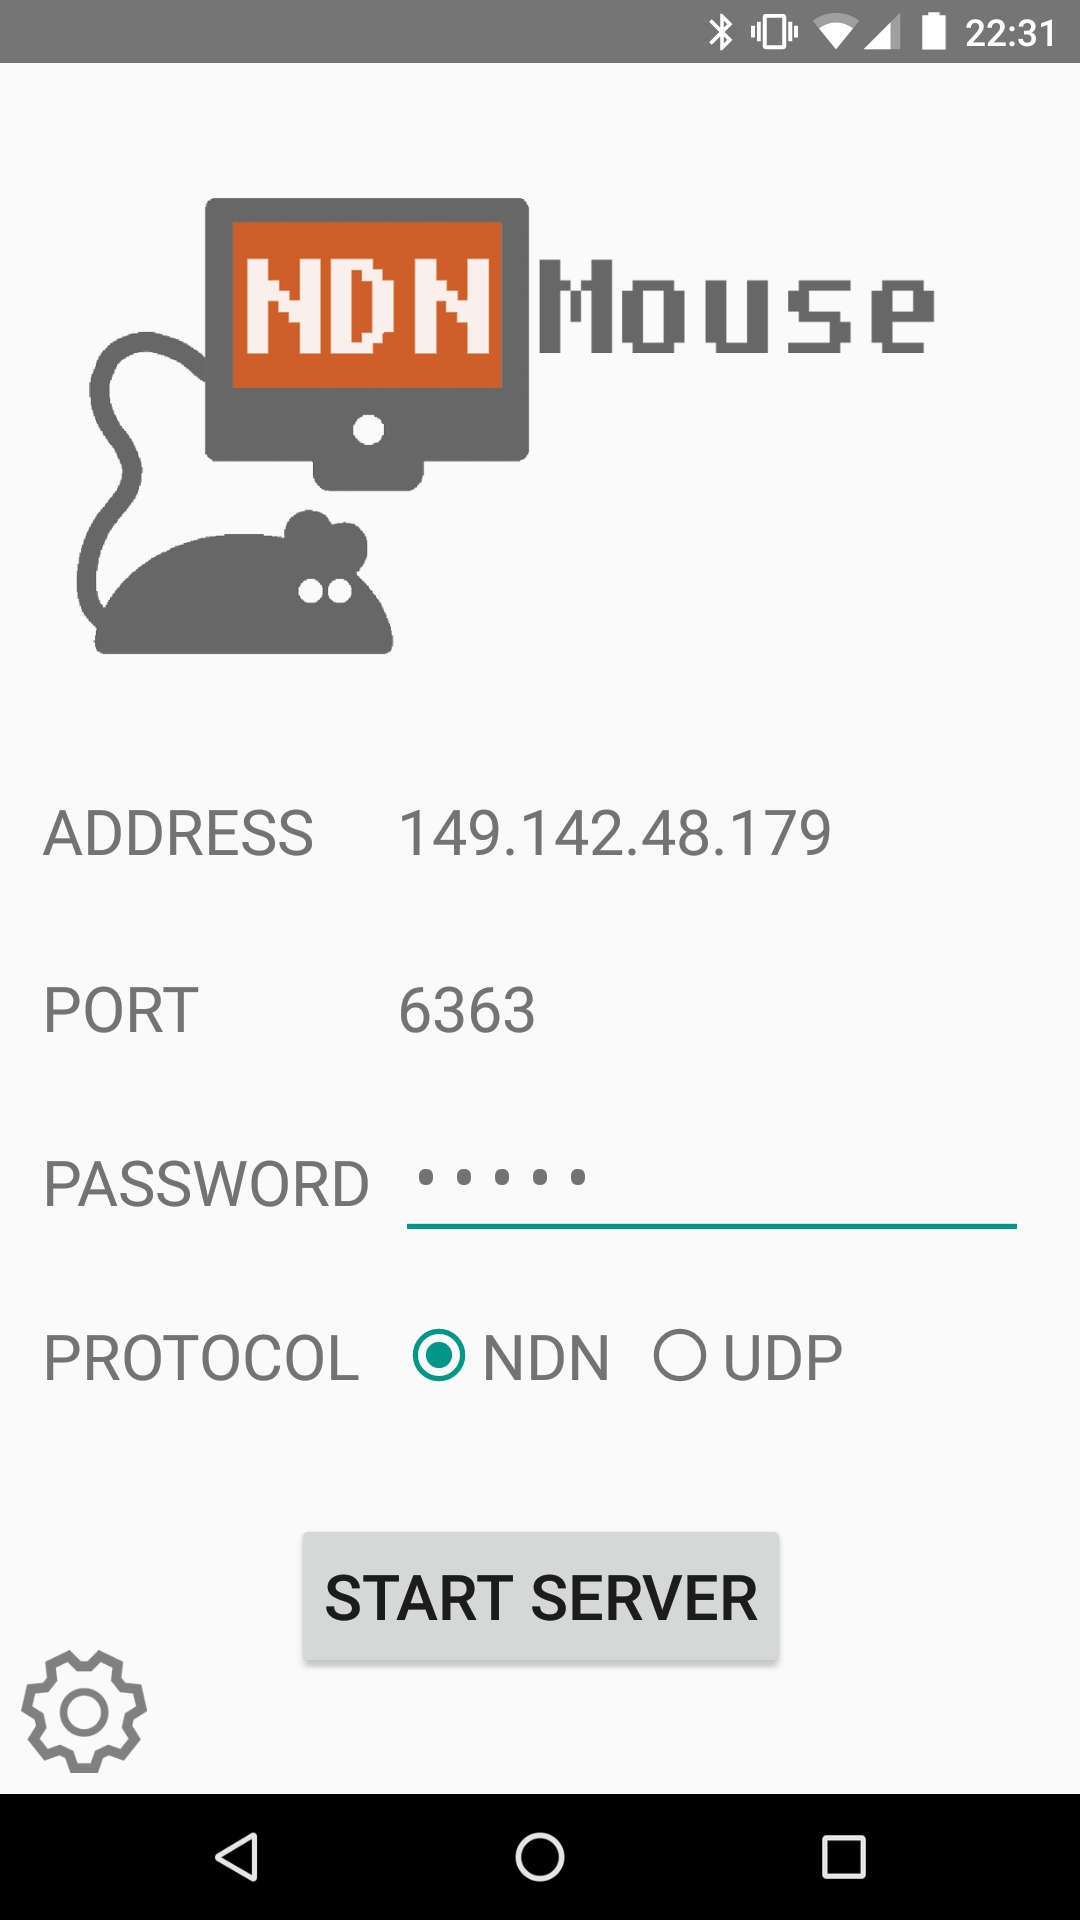
\includegraphics[width=6cm]{screenshots/start}
	\caption{Start screen}
\end{figure}

\begin{figure}[hp]
	\hypertarget{fig:settings}{}
	\centering
	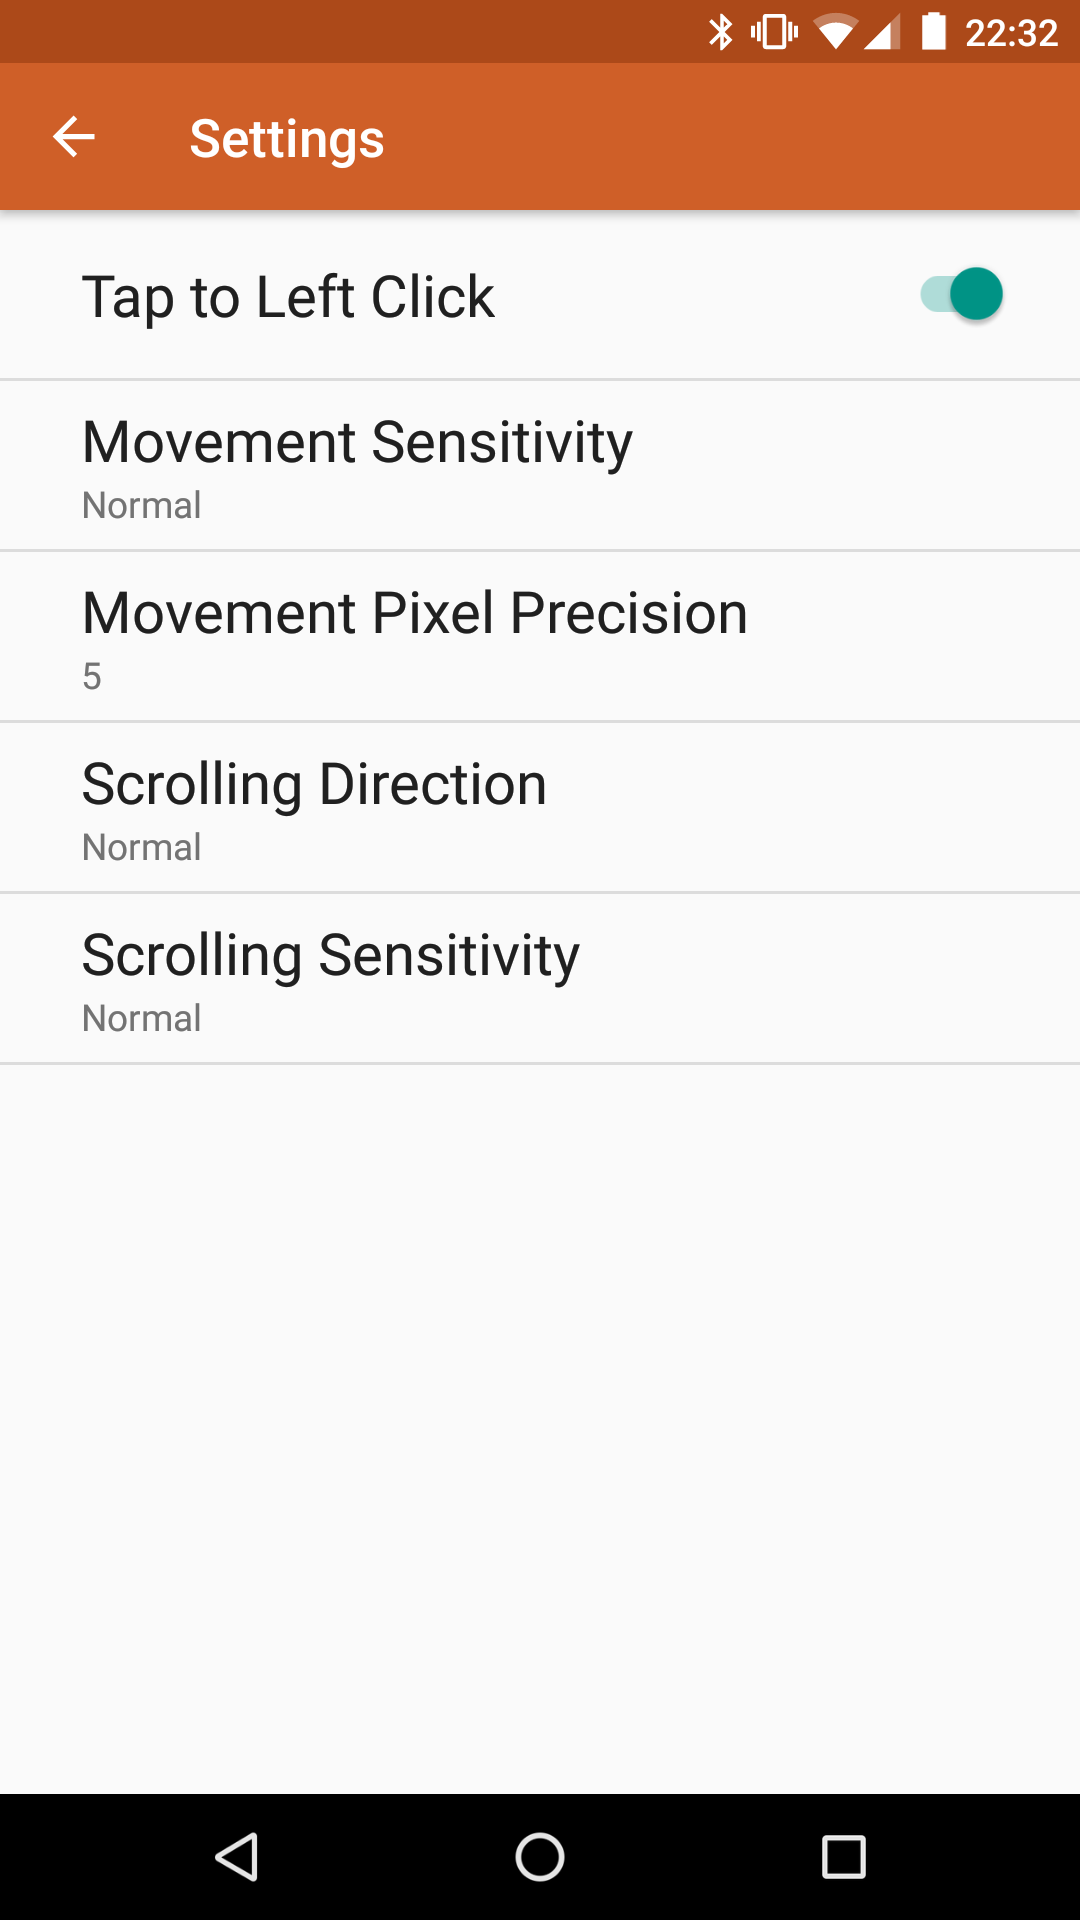
\includegraphics[width=6cm]{screenshots/settings}
	\caption{Settings screen}
\end{figure}

\begin{figure}[hp]
	\hypertarget{fig:touchpad}{}
	\centering
	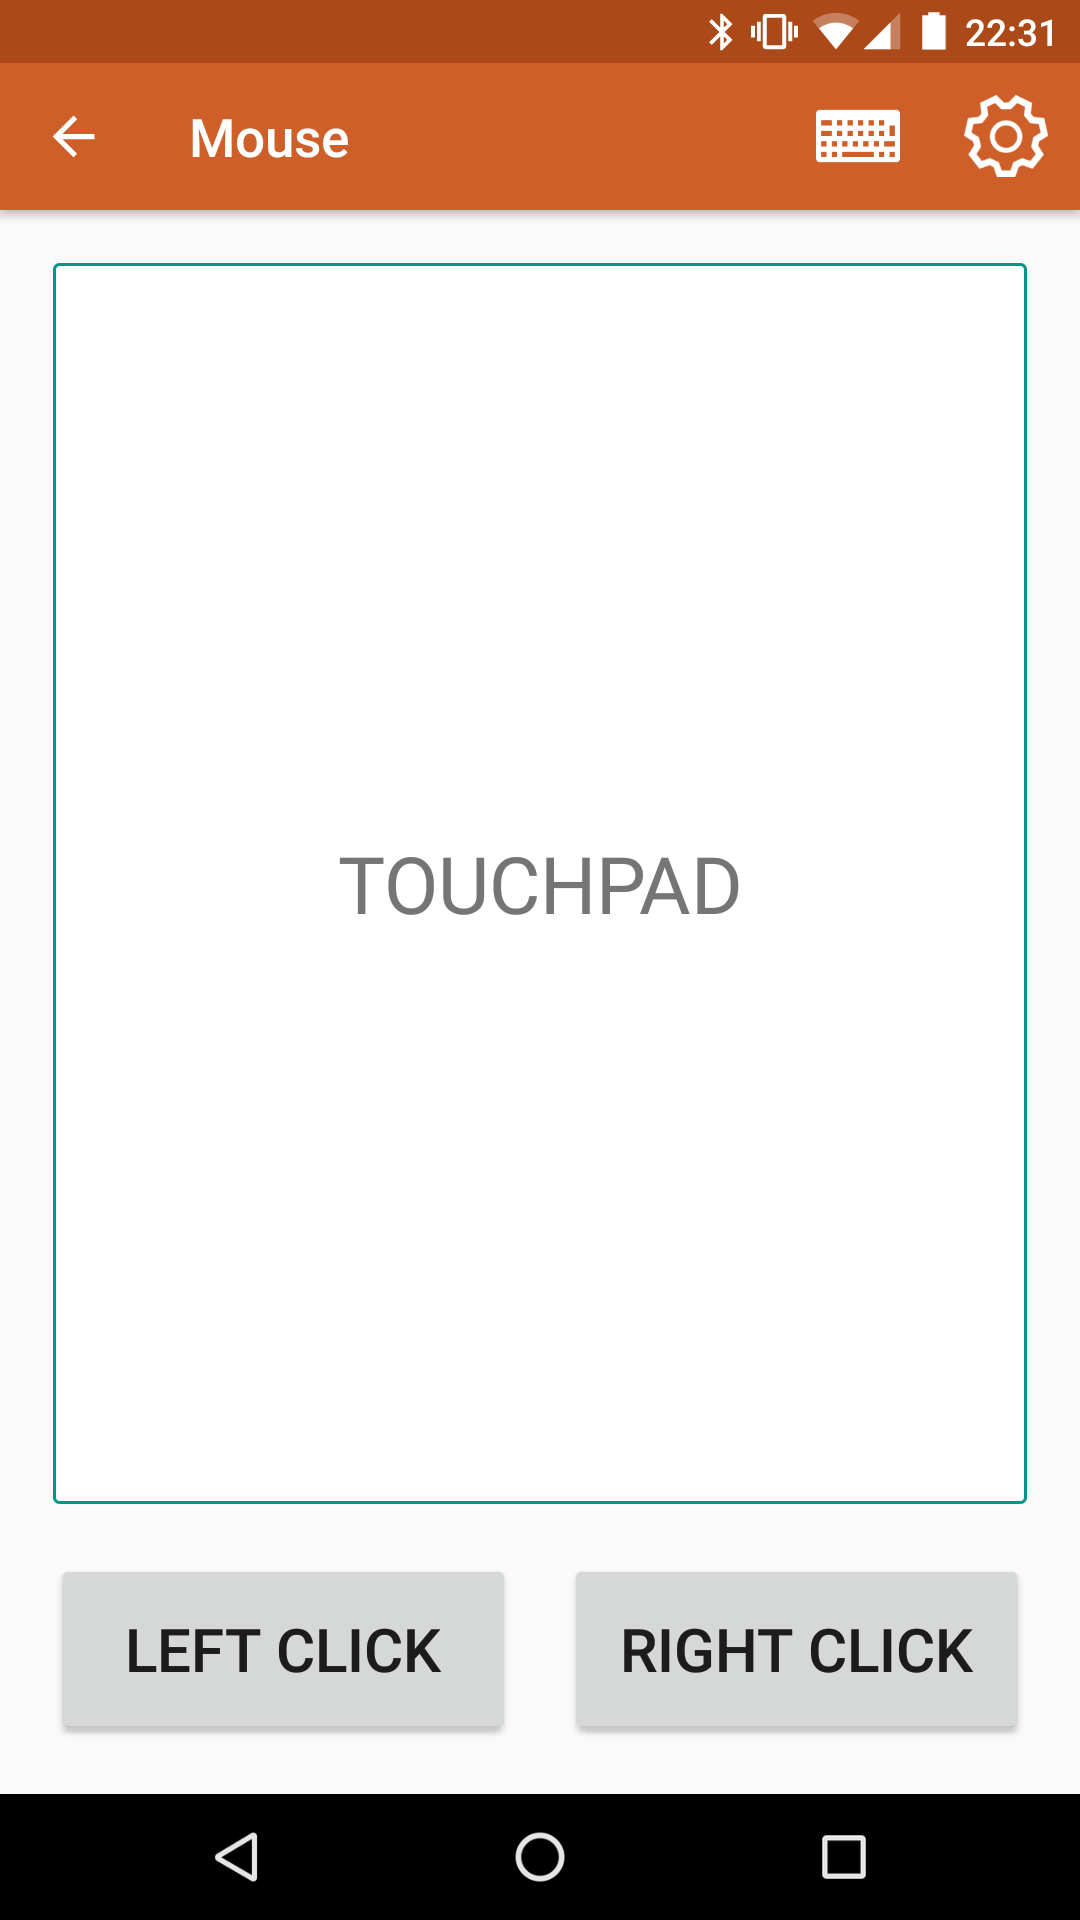
\includegraphics[width=6cm]{screenshots/touchpad}
	\caption{Touchpad screen}
\end{figure}

\begin{figure}[hp]
	\hypertarget{fig:keyboard}{}
	\centering
	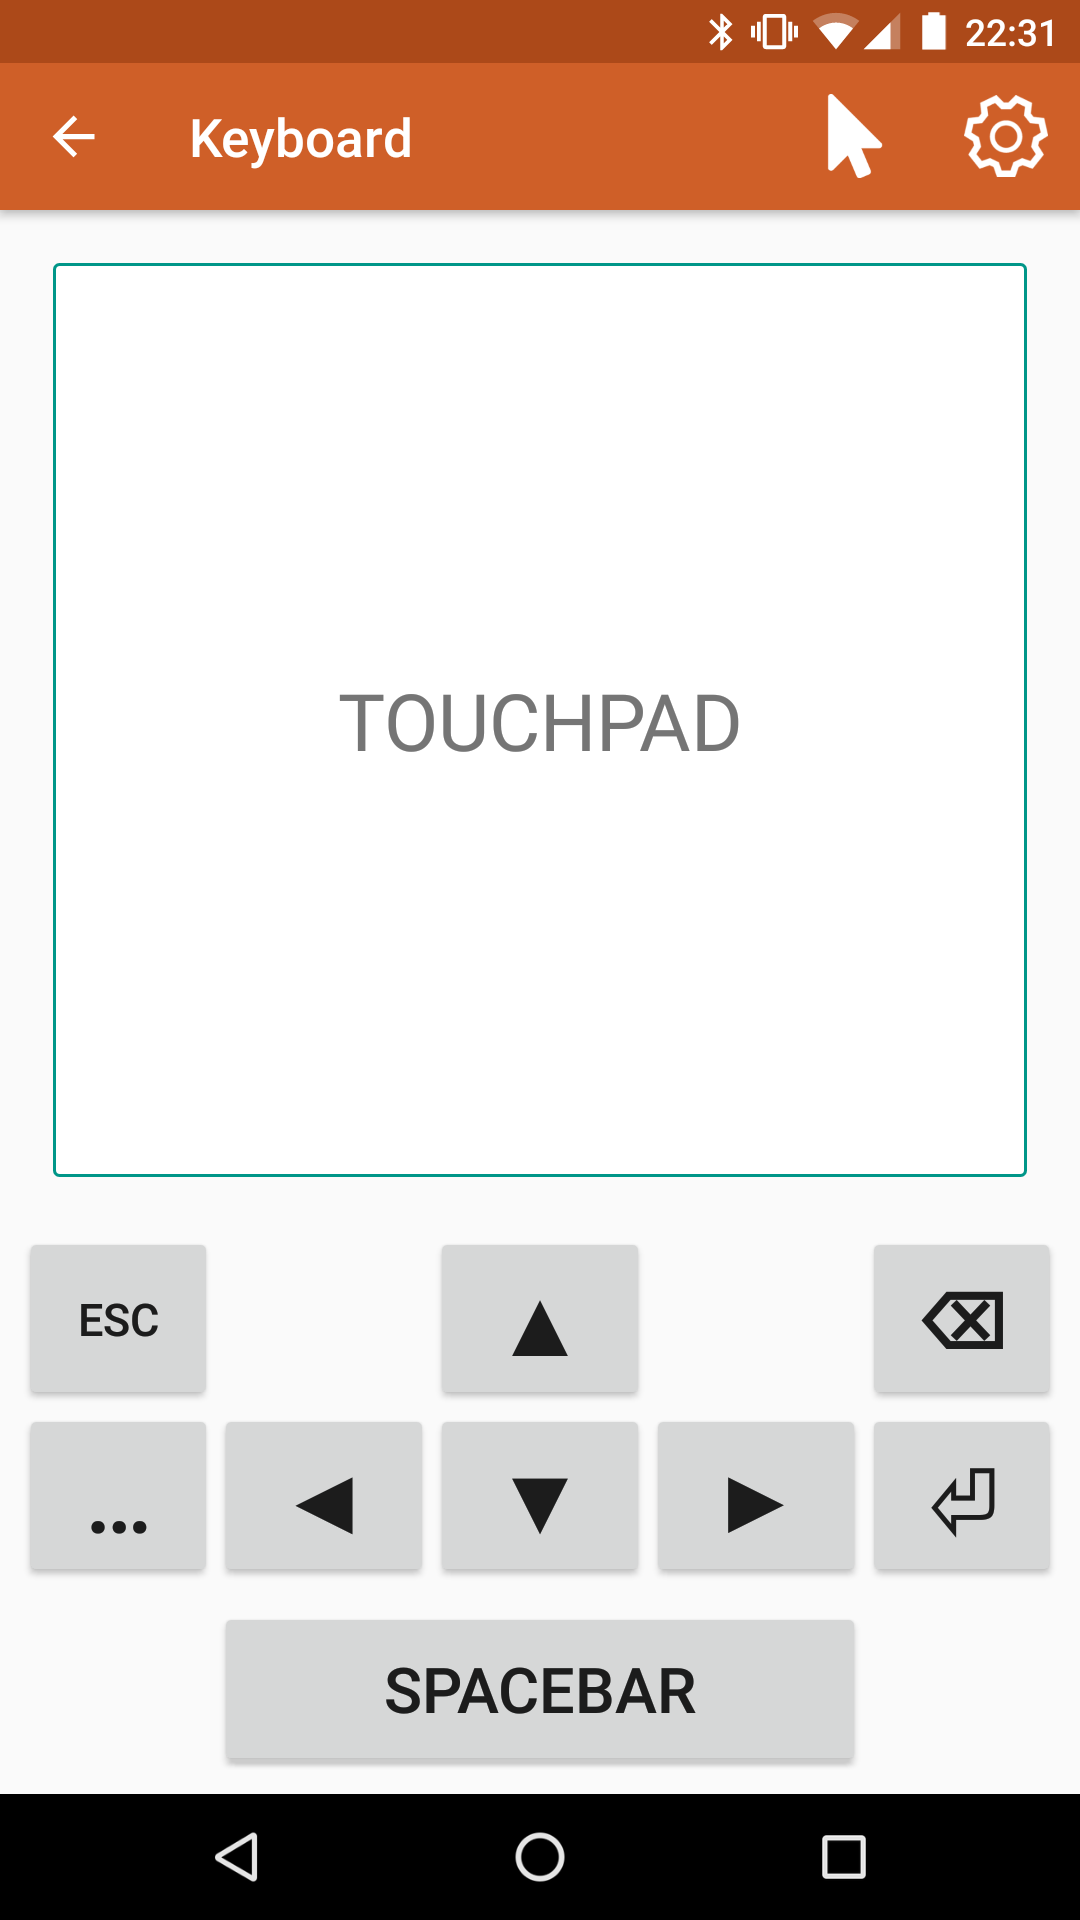
\includegraphics[width=6cm]{screenshots/keyboard}
	\caption{Keyboard screen}
\end{figure}

\begin{figure}[hp]
	\hypertarget{fig:custom\_type\_message}{}
	\centering
	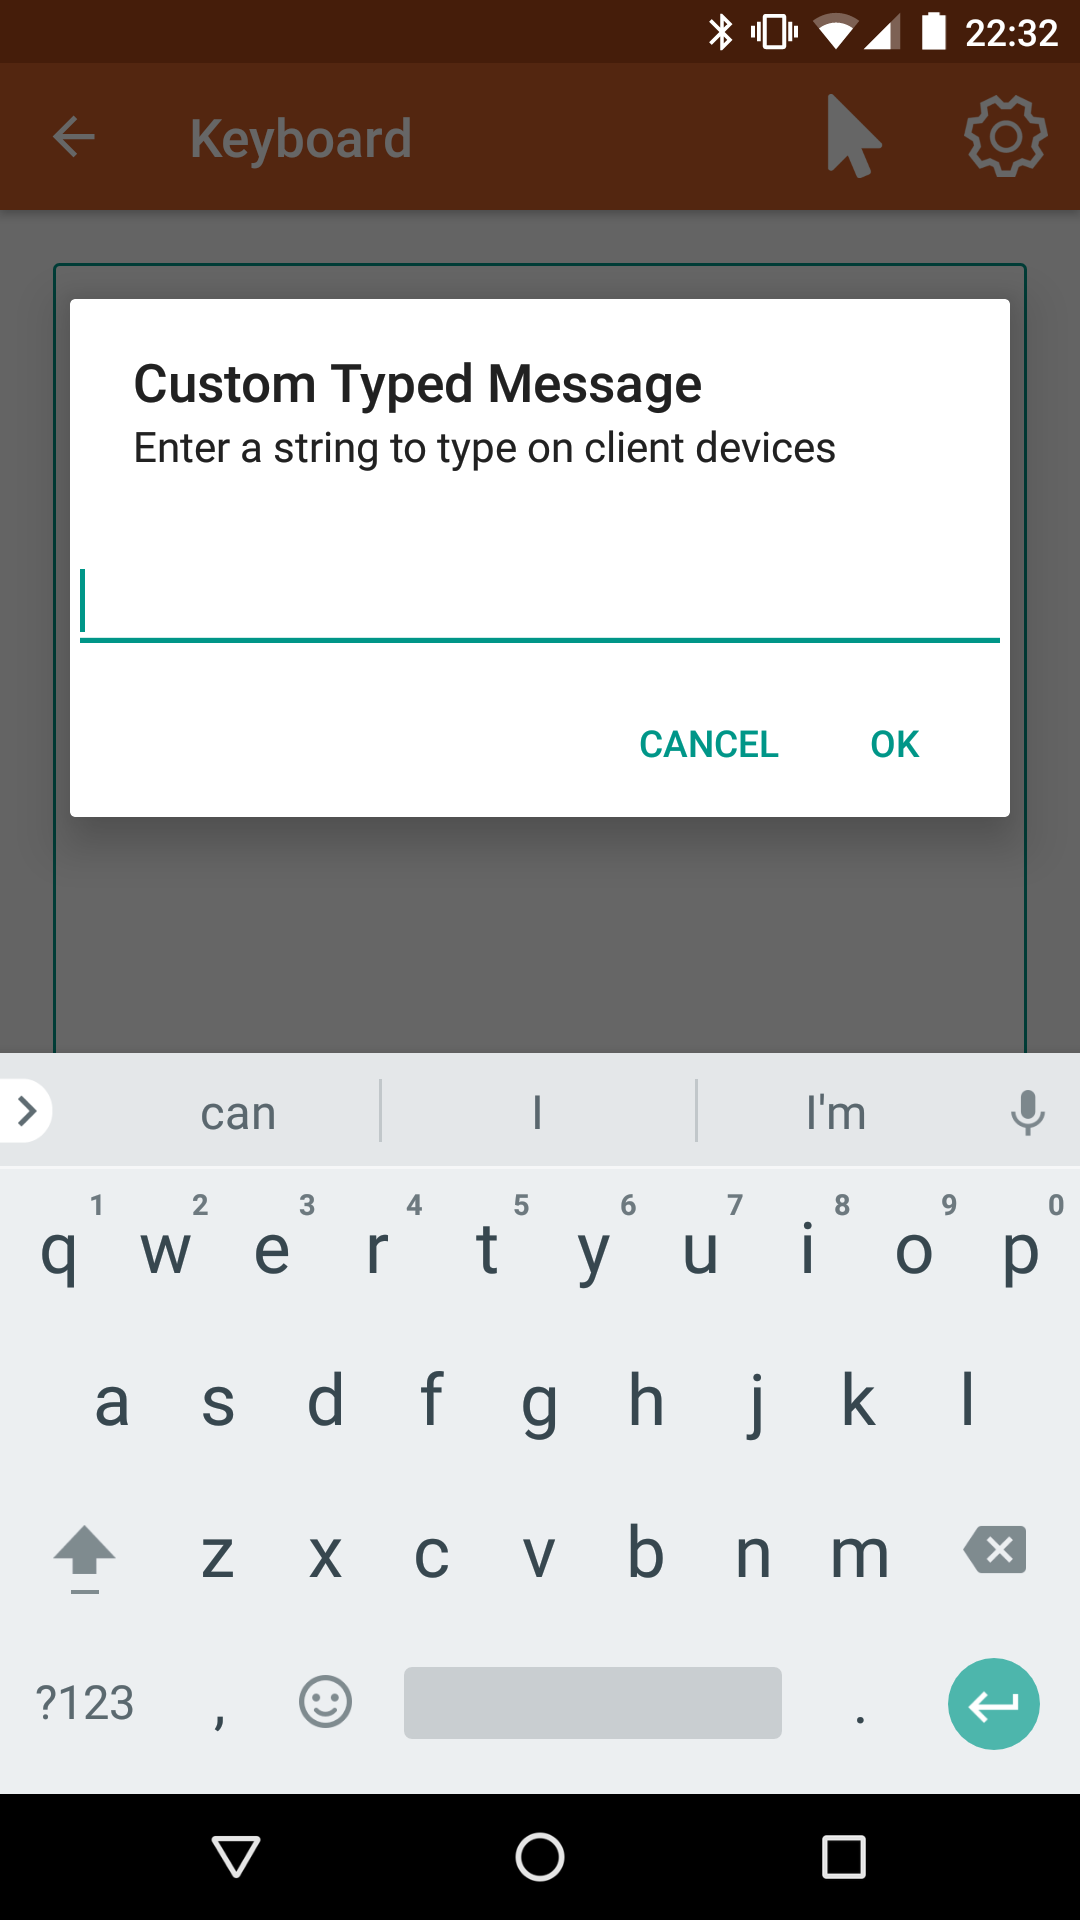
\includegraphics[width=6cm]{screenshots/custom_type_message}
	\caption{Custom typed message entry}
\end{figure}

\begin{figure*}[hp]
	\hypertarget{fig:client1}{}
	\centering
	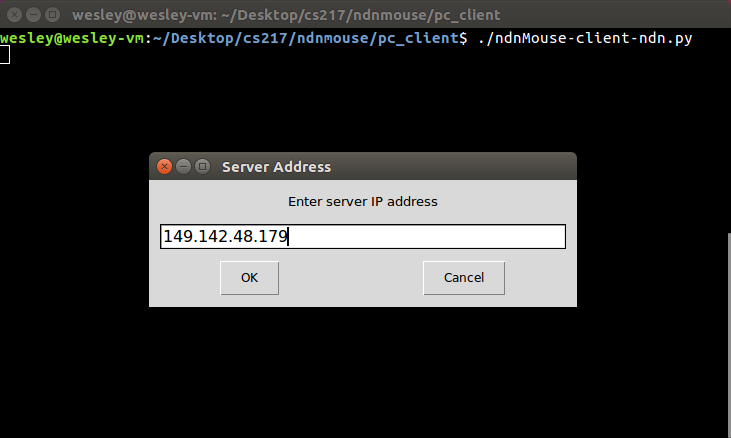
\includegraphics[width=11cm]{screenshots/client1}
	\caption{PC program IP address entry}
\end{figure*}

\begin{figure*}[hp]
	\hypertarget{fig:client2}{}
	\centering
	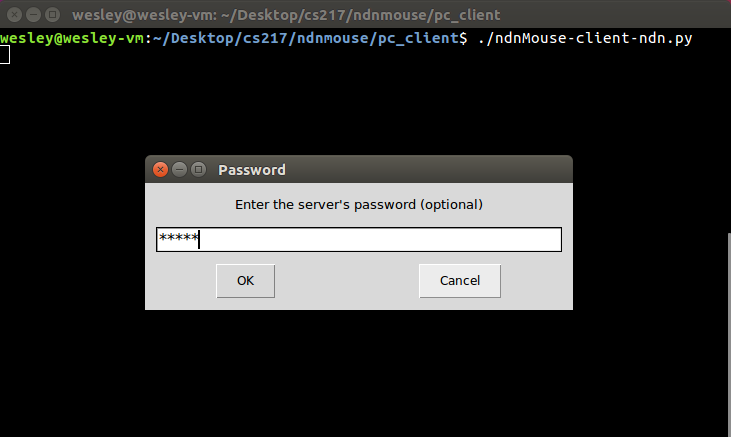
\includegraphics[width=11cm]{screenshots/client2}
	\caption{PC program password entry}
\end{figure*}

\begin{figure*}[hp]
	\hypertarget{fig:client3}{}
	\centering
	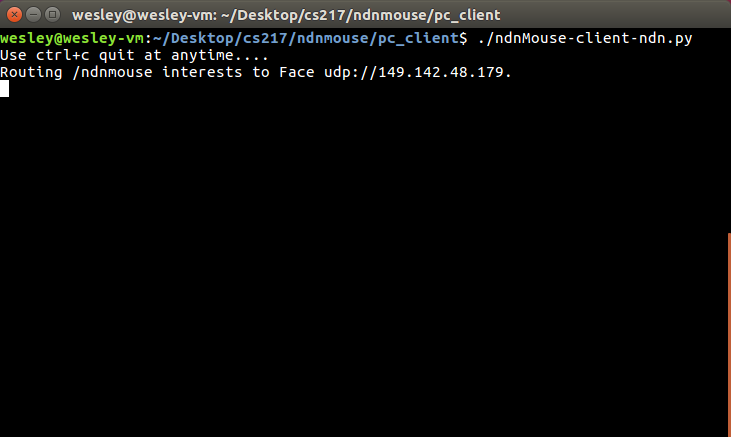
\includegraphics[width=11cm]{screenshots/client3}
	\caption{PC program running}
\end{figure*}

\end{document}